\documentclass[11pt,a4paper]{article}
\usepackage[utf8]{inputenc}
\usepackage[vietnamese]{babel}
\usepackage{amsmath,amssymb}
\usepackage[version=4]{mhchem}
\usepackage{geometry}
\geometry{top=1.5cm,bottom=1.2cm,left=1.4cm,right=1.4cm,headheight=28pt,headsep=12pt,footskip=18pt}
\usepackage{graphicx}
\usepackage{xcolor}
\usepackage{tabularx}
\usepackage{array}
\usepackage{colortbl}
\usepackage{tikz}
\usepackage{chemfig}
\usepackage{fancyhdr}
\usepackage{enumitem}
\usepackage{multido}
\usepackage{tcolorbox}

\definecolor{hfRed}{HTML}{D32F2F}
\definecolor{hfGreen}{HTML}{8BC390}
\definecolor{mainGreen}{HTML}{2E7D32}
\definecolor{solBlue}{HTML}{1565C0}
\definecolor{tableGreen}{HTML}{E8F5E9}

\usepackage{ex_test}

\pagestyle{fancy}
\fancyhf{}
\renewcommand{\headrulewidth}{0.75pt}
\renewcommand{\headrule}{\hbox to\headwidth{\color{hfGreen}\leaders\hrule height \headrulewidth\hfill}}
\renewcommand{\footrulewidth}{0.75pt}
\renewcommand{\footrule}{\hbox to\headwidth{\color{hfGreen}\leaders\hrule height \footrulewidth\hfill}}

\fancyhead[L]{\small\itshape\color{hfRed}Tài liệu lưu hành nội bộ}
\fancyhead[R]{\small\color{hfRed}Thầy \textbf{TRẦN VĂN THẠNH} - 0777.470.803}

\fancyfoot[L]{\footnotesize\itshape\color{hfRed}CS1: 6/15 Nguyễn Hoàng, P. Kim Long, TP Huế \quad|\quad CS2: 24 Đặng Thái Thân, TP Huế}
\fancyfoot[R]{\small\textbf{\color{hfRed}Trang \thepage}}

\setlength{\parindent}{0pt}
\setlength{\parskip}{2pt}

\begin{document}

\begin{minipage}[t]{0.48\textwidth}
\textbf{SỞ GD - ĐT THÀNH PHỐ HUẾ}\\
\textbf{TRƯỜNG THPT ĐẶNG HUY TRỨ}\\
\textit{ĐỀ CHÍNH THỨC}\\
\textit{(Đề thi có 03 trang)}
\end{minipage}
\hfill
\begin{minipage}[t]{0.48\textwidth}
\raggedleft
\textbf{\color{hfRed}KIỂM TRA CUỐI KỲ I}\\
\textbf{NĂM HỌC 2025 -- 2026}\\
\textbf{MÔN: HÓA HỌC -- LỚP 11}\\
\textit{Thời gian làm bài: 45 phút (không kể thời gian phát đề)}\\
\textbf{MÃ ĐỀ: 102}
\end{minipage}

\vspace{4pt}
\noindent
\textit{Họ và tên học sinh:} \dotfill \textit{Lớp:} \dotfill \textit{SBD:} \dotfill

\vspace{3pt}
\noindent
\textit{\footnotesize Cho biết nguyên tử khối của các nguyên tố: $\ce{C} = 12; \ce{H} = 1; \ce{O} = 16; \ce{Ba} = 137; \ce{S} = 32$.}

\vspace{3pt}
\hrule color{hfGreen} height 0.5pt

\vspace{6pt}
\begin{center}
{\large\bfseries\color{hfRed} BẢNG ĐÁP ÁN RÚT GỌN (DÀNH CHO GIÁO VIÊN - MÃ ĐỀ 102)}
\end{center}

\vspace{4pt}
{\bfseries\color{mainGreen} 1. PHẦN I: TRẮC NGHIỆM NHIỀU PHƯƠNG ÁN LỰA CHỌN (4,0 ĐIỂM)}

\vspace{2pt}
\begin{center}
\renewcommand{\arraystretch}{1.2}
\begin{tabular}{|c|c|c|c|c|c|c|c|c|}
\hline
\rowcolor{tableGreen}
\textbf{Câu} & \textbf{1} & \textbf{2} & \textbf{3} & \textbf{4} & \textbf{5} & \textbf{6} & \textbf{7} & \textbf{8} \\ \hline
\textbf{Đ/A} & \textbf{\color{hfRed}C} & \textbf{\color{hfRed}C} & \textbf{\color{hfRed}B} & \textbf{\color{hfRed}C} & \textbf{\color{hfRed}B} & \textbf{\color{hfRed}A} & \textbf{\color{hfRed}B} & \textbf{\color{hfRed}D} \\ \hline
\rowcolor{tableGreen}
\textbf{Câu} & \textbf{9} & \textbf{10} & \textbf{11} & \textbf{12} & \textbf{13} & \textbf{14} & \textbf{15} & \textbf{16} \\ \hline
\textbf{Đ/A} & \textbf{\color{hfRed}A} & \textbf{\color{hfRed}D} & \textbf{\color{hfRed}D} & \textbf{\color{hfRed}A} & \textbf{\color{hfRed}D} & \textbf{\color{hfRed}A} & \textbf{\color{hfRed}C} & \textbf{\color{hfRed}D} \\ \hline
\end{tabular}
\end{center}

\vspace{4pt}
{\bfseries\color{mainGreen} 2. PHẦN II: TRẮC NGHIỆM ĐÚNG SAI (2,0 ĐIỂM)}

\vspace{2pt}
\begin{center}
\renewcommand{\arraystretch}{1.2}
\begin{tabular}{|c|p{7.5cm}|c|c|c|c|}
\hline
\rowcolor{tableGreen}
\textbf{Câu} & \textbf{Nội dung câu hỏi} & \textbf{Lệnh a} & \textbf{Lệnh b} & \textbf{Lệnh c} & \textbf{Lệnh d} \\ \hline
\textbf{Câu 1} & Sulfur dioxide ($\ce{SO2}$) và môi trường & \textbf{\color{hfRed}ĐÚNG} & \textbf{\color{hfRed}ĐÚNG} & \textbf{\color{hfRed}ĐÚNG} & \textbf{SAI} \\ \hline
\textbf{Câu 2} & Cấu tạo và tính chất hợp chất hữu cơ (1)-(5) & \textbf{SAI} & \textbf{\color{hfRed}ĐÚNG} & \textbf{\color{hfRed}ĐÚNG} & \textbf{SAI} \\ \hline
\end{tabular}
\end{center}

\vspace{4pt}
{\bfseries\color{mainGreen} 3. PHẦN III: TRẮC NGHIỆM TRẢ LỜI NGẮN (1,0 ĐIỂM)}

\vspace{2pt}
\begin{center}
\renewcommand{\arraystretch}{1.2}
\begin{tabular}{|c|c|c|c|c|}
\hline
\rowcolor{tableGreen}
\textbf{Câu hỏi} & \textbf{Câu 1} & \textbf{Câu 2} & \textbf{Câu 3} & \textbf{Câu 4} \\ \hline
\textbf{Đáp án} & \textbf{\color{hfRed}3} & \textbf{\color{hfRed}0,15} & \textbf{\color{hfRed}3} & \textbf{\color{hfRed}11,9} \\ \hline
\end{tabular}
\end{center}

\vspace{4pt}
{\bfseries\color{mainGreen} 4. TÓM TẮT ĐÁP SỐ PHẦN TỰ LUẬN (3,0 ĐIỂM)}

\vspace{2pt}
\begin{center}
\renewcommand{\arraystretch}{1.2}
\begin{tabular}{|c|c|p{13.2cm}|}
\hline
\rowcolor{tableGreen}
\textbf{Câu} & \textbf{Điểm} & \textbf{Đáp số cốt lõi \& Hướng dẫn chấm} \\ \hline
\textbf{Câu 1} & 1,0 đ & a) $\ce{2KOH + H2SO4 -> K2SO4 + 2H2O}$ (0,25 đ)\\
& & b) $\ce{3H2SO4(l) + Fe2O3 -> Fe2(SO4)3 + 3H2O}$ (0,25 đ)\\
& & c) $\ce{4NO2 + O2 + 2H2O -> 4HNO3}$ (0,25 đ)\\
& & d) $\ce{NH4Cl + NaOH -> NaCl + NH3 ^ + H2O}$ (0,25 đ) \\ \hline
\textbf{Câu 2} & 1,0 đ & 1) $x : y : z = \frac{78{,}94}{12} : \frac{10{,}53}{1} : \frac{10{,}53}{16} = 6{,}578 : 10{,}53 : 0{,}658 \approx 10 : 16 : 1 \Rightarrow \ce{C10H16O}$ (0,5 đ)\\
& & b) CTPT có dạng $(\ce{C10H16O})_n \Rightarrow M = 152n$. Phổ MS có $[M^+]$ tại $m/z = 152 \Rightarrow n = 1 \Rightarrow \ce{C10H16O}$ (0,5 đ) \\ \hline
\textbf{Câu 3} & 1,0 đ & $\ce{5SO2 + 2KMnO4 + 2H2O -> K2SO4 + 2MnSO4 + 2H2SO4}$.\\
& & $n_{\ce{KMnO4}} = 6{,}25\cdot 10^{-5}\text{ mol} \Rightarrow n_{\ce{SO2(10 mL)}} = 1{,}5625\cdot 10^{-4}\text{ mol} \Rightarrow n_{\ce{SO2(500 mL)}} = 7{,}8125\cdot 10^{-3}\text{ mol}$.\\
& & $m_{\ce{S}} = 7{,}8125\cdot 10^{-3} \times 32 = 0{,}25\text{ g} \Rightarrow \%m_{\ce{S}} = \frac{0{,}25}{100{,}0}\times 100\% = 0{,}25\% \le 0{,}3\%$ (Đạt chuẩn). \\ \hline
\end{tabular}
\end{center}

\vspace{4pt}
\hrule color{hfGreen} height 0.5pt

\vspace{6pt}
{\large\bfseries\color{mainGreen} A. TRẮC NGHIỆM (7,0 điểm)}

\vspace{3pt}
{\bfseries\color{mainGreen} Phần I: Trắc nghiệm nhiều lựa chọn (4,0 điểm).}
\textit{Học sinh trả lời từ câu 1 đến câu 16. Mỗi câu hỏi học sinh chỉ chọn một phương án.}
\vspace{4pt}
\begin{ex}
Công thức phân tử chất hữu cơ \textbf{không thể} cho ta biết:
\choice
{Tỉ lệ giữa các nguyên tố trong hợp chất}
{Số lượng các nguyên tố trong hợp chất.}
{{\textbf{\color{hfRed}Cấu trúc phân tử hợp chất hữu cơ.}}}
{Hàm lượng mỗi nguyên tố trong hợp chất.}
\loigiai{
Công thức phân tử cho biết số lượng nguyên tử mỗi nguyên tố trong một phân tử hợp chất hữu cơ, từ đó xác định được tỉ lệ nguyên tố, khối lượng phân tử và thành phần phần trăm khối lượng các nguyên tố. CTPT không cho biết trật tự liên kết và cấu trúc không gian (phải dùng CTCT).
}
\end{ex}
\begin{ex}
Cho phổ khối lượng của một hợp chất hữu cơ A như hình vẽ:
\begin{center}
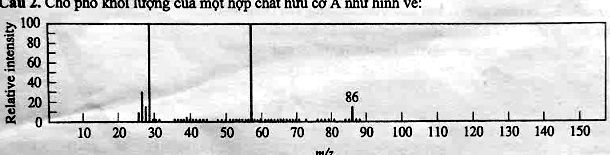
\includegraphics[width=0.75\textwidth]{images_danghuytru_ma102/ms_cau2_clean.png}
\end{center}
Hợp chất hữu cơ A có thể là
\choice
{\ce{C4H8O2}.}
{\ce{CH2Cl2}.}
{{\textbf{\color{hfRed}\ce{C4H6O2}.}}}
{\ce{C7H8}.}
\loigiai{
Trên phổ khối lượng (MS), peak ion phân tử $[M^+]$ có $m/z = 86 \Rightarrow M_A = 86\text{ g/mol}$.
- \ce{C4H8O2}: $M = 88$.
- \ce{CH2Cl2}: $M = 85$.
- \ce{C4H6O2}: $M = 12\times 4 + 6 + 16\times 2 = 86$ (thỏa mãn).
- \ce{C7H8}: $M = 92$.
Vậy A có thể là \ce{C4H6O2}.
}
\end{ex}
\begin{ex}
Dung dịch nào sau đây có $\text{pH} \approx 7$?
\choice
{\ce{NaOH}.}
{{\textbf{\color{hfRed}\ce{NaCl}.}}}
{\ce{HNO3}.}
{\ce{H2SO4}.}
\loigiai{
\ce{NaCl} là muối tạo bởi base mạnh và acid mạnh, không bị thủy phân nên có môi trường trung tính ($\text{pH} \approx 7$).
}
\end{ex}
\begin{ex}
Khi phản ứng với kim loại, Sulfur thể hiện tính chất gì?
\choice
{tính khử.}
{tính lưỡng tính.}
{{\textbf{\color{hfRed}tính oxi hóa.}}}
{vừa tính oxi hóa, vừa tính khử.}
\loigiai{
Khi phản ứng với kim loại (ví dụ $\ce{Fe + S -> FeS}$), số oxi hóa của sulfur giảm từ 0 xuống -2, thể hiện tính oxi hóa.
}
\end{ex}
\begin{ex}
Phú dưỡng là hiện tượng môi trường nước (ao, hồ, sông) bị dư thừa quá mức các chất dinh dưỡng, chủ yếu là Nitơ (N) và Photpho (P), do nước thải nông nghiệp, sinh hoạt, công nghiệp đổ vào, dẫn đến sự phát triển bùng nổ của tảo (nở hoa) và vi sinh vật, gây thiếu oxy, chết cá, làm suy giảm chất lượng nước và mất cân bằng sinh thái.

Cách nào sau đây \textbf{không đúng} khi xử lí hiện tượng phú dưỡng trong các ao hồ?
\choice
{Sử dụng phân bón hợp lý trong nông nghiệp.}
{{\textbf{\color{hfRed}Phun thuốc diệt cỏ để diệt tảo.}}}
{Xử lý nước thải trước khi xả ra môi trường.}
{Nạo vét bùn, khơi thông dòng chảy cho ao, hồ, sông.}
\loigiai{
Phun thuốc diệt cỏ vào ao hồ sẽ gây độc hại nghiêm trọng cho hệ sinh thái thủy sinh, làm chết các loài thủy sản và ô nhiễm nguồn nước nặng hơn.
}
\end{ex}
\begin{ex}
Để tách các chất lỏng ra khỏi hỗn hợp các chất có nhiệt độ sôi khác nhau, nhằm thu được chất lỏng tinh khiết hơn là phương pháp nào sau đây?
\choice
{{\textbf{\color{hfRed}Phương pháp chưng cất.}}}
{Phương pháp chiết}
{Sắc kí cột.}
{Phương pháp kết tinh.}
\loigiai{
Phương pháp chưng cất dùng để tách các chất lỏng có nhiệt độ sôi khác nhau.
}
\end{ex}
\begin{ex}
\ce{HNO3} tinh khiết là chất lỏng không màu, nhưng dung dịch \ce{HNO3} để lâu thường chuyển sang màu vàng là do
\choice
{khi để lâu thì \ce{HNO3} bị khử bởi các chất của môi trường}
{{\textbf{\color{hfRed}dung dịch \ce{HNO3} có hoà tan một lượng nhỏ \ce{NO2}.}}}
{dung dịch \ce{HNO3} có tính oxi hoá mạnh.}
{\ce{HNO3} tan nhiều trong nước.}
\loigiai{
Dung dịch \ce{HNO3} bị phân hủy một phần dưới ánh sáng hoặc nhiệt độ tạo khí \ce{NO2}: $\ce{4HNO3 -> 4NO2 ^ + O2 ^ + 2H2O}$. Khí \ce{NO2} màu nâu đỏ hòa tan một lượng nhỏ vào dung dịch làm dung dịch có màu vàng.
}
\end{ex}
\begin{ex}
Phản ứng hóa học của các hợp chất hữu cơ có đặc điểm là:
\choice
{thường xảy ra rất nhanh và cho một sản phẩm duy nhất.}
{thường xảy ra rất chậm, nhưng hoàn toàn, không theo một hướng xác định.}
{thường xảy ra rất nhanh, không hoàn toàn, không theo một hướng nhất định.}
{{\textbf{\color{hfRed}thường xảy ra chậm, không hoàn toàn, không theo một hướng nhất định.}}}
\loigiai{
Liên kết cộng hóa trị trong chất hữu cơ bền vững và kém phân cực nên phản ứng thường xảy ra chậm, không hoàn toàn và sinh ra hỗn hợp sản phẩm (không theo một hướng nhất định).
}
\end{ex}
\begin{ex}
Trong các phát biểu sau đây, phát biểu nào \textbf{đúng} khi một hệ ở trạng thái cân bằng?
\choice
{{\textbf{\color{hfRed}Nồng độ của các chất trong hệ không đổi.}}}
{Phản ứng thuận đã dừng.}
{Nồng độ chất tham gia và sản phẩm bằng nhau.}
{Phản ứng nghịch đã dừng.}
\loigiai{
Cân bằng hóa học là cân bằng động ($v_t = v_n > 0$), nồng độ các chất trong hệ không thay đổi theo thời gian.
}
\end{ex}
\begin{ex}
Tính chất nào sau đây \textbf{không phải} tính chất của dung dịch sulfuric acid đặc?
\choice
{Tính háo nước.}
{Tính oxi hóa.}
{Tính acid.}
{{\textbf{\color{hfRed}Tính khử.}}}
\loigiai{
Trong \ce{H2SO4}, nguyên tố sulfur có số oxi hóa cao nhất là +6 nên acid sulfuric đặc có tính oxi hóa mạnh, tính acid và tính háo nước; không có tính khử.
}
\end{ex}
\begin{ex}
Phát biểu nào sau đây \textbf{đúng} khi nói về sự điện li?
\choice
{Sự điện li thực chất là quá trình oxi hoá – khử.}
{Sự điện li quá trình hòa tan một chất vào nước tạo thành dung dịch.}
{Sự điện li quá trình phân li một chất dưới tác dụng của dòng điện.}
{{\textbf{\color{hfRed}Sự điện li là quá trình phân li một chất trong nước thành ion.}}}
\loigiai{
Theo định nghĩa: Sự điện li là quá trình phân li các chất khi tan trong nước thành các ion.
}
\end{ex}
\begin{ex}
Xác định công thức cấu tạo thu gọn của hợp chất sau:
\begin{center}
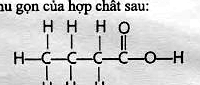
\includegraphics[width=0.35\textwidth]{images_danghuytru_ma102/ctct_cau12_clean.png}
\end{center}
\choice
{{\textbf{\color{hfRed}\ce{CH3CH2CH2COOH}.}}}
{\ce{CH3CH2CH2OH}.}
{\ce{CH3CH2CHOHCHO}.}
{\ce{CH3CH2COOH}.}
\loigiai{
Công thức có chuỗi 4 carbon: $\ce{CH3-CH2-CH2-COOH}$ (butanoic acid).
}
\end{ex}
\begin{ex}
Cho chất X có công thức cấu tạo thu gọn như sau: $\ce{CH3-COOH}$. Phân tử chất X chứa nhóm chức gì?
\choice
{-COO-}
{-CO-}
{-CHO}
{{\textbf{\color{hfRed}-COOH}}}
\loigiai{
Phân tử $\ce{CH3COOH}$ chứa nhóm chức carboxyl (-COOH) của carboxylic acid.
}
\end{ex}
\begin{ex}
Liên kết hoá học trong phân tử \ce{NH3} là liên kết
\choice
{{\textbf{\color{hfRed}cộng hoá trị có cực.}}}
{phối trí.}
{cộng hoá trị không cực.}
{ion.}
\loigiai{
Liên kết N-H trong phân tử ammonia (\ce{NH3}) là liên kết cộng hóa trị có cực do chênh lệch độ âm điện giữa N và H.
}
\end{ex}
\begin{ex}
Cho dung dịch \ce{HNO3} tác dụng với các chất sau: \ce{NH3}, \ce{CaCO3}, \ce{Ag}, \ce{NaOH}. Theo Bronsted, số phản ứng trong đó \ce{HNO3} đóng vai trò acid là
\choice
{1.}
{4.}
{{\textbf{\color{hfRed}3.}}}
{2.}
\loigiai{
Theo Brønsted, acid là chất cho proton ($H^+$). \ce{HNO3} cho $H^+$ trong 3 phản ứng với \ce{NH3}, \ce{CaCO3}, \ce{NaOH}. Còn phản ứng với Ag là phản ứng oxi hóa - khử.
}
\end{ex}
\begin{ex}
Glucose là hợp chất hữu cơ có nhiều trong các loại quả chín, đặc biệt là quả nho. Công thức phân tử của glucose là \ce{C6H12O6}. Công thức đơn giản nhất của glucose là
\choice
{\ce{CHO2}.}
{\ce{CH3O}.}
{\ce{C3H4O3}.}
{{\textbf{\color{hfRed}\ce{CH2O}.}}}
\loigiai{
Tỉ lệ số nguyên tử trong \ce{C6H12O6}: $C : H : O = 6 : 12 : 6 = 1 : 2 : 1 \Rightarrow \ce{CH2O}$.
}
\end{ex}

\vspace{6pt}
{\bfseries\color{mainGreen} Phần II: Trắc nghiệm dạng Đúng/Sai (2,0 điểm).}
\textit{Học sinh trả lời từ câu 1 đến câu 2. Trong mỗi ý a), b), c), d) ở mỗi câu, học sinh chọn đúng hoặc sai.}
\vspace{4pt}
\begin{ex}
Sulfur dioxide ($\ce{SO2}$) là một chất khí không màu, có mùi hăng đặc trưng, nặng hơn không khí và có mặt trong không khí từ các nguồn khác nhau.
\choiceTF
{\True Khí $\ce{SO2}$ là một trong những tác nhân gây ô nhiễm môi trường và viêm đường hô hấp ở người, ...}
{\True Để giảm thải $\ce{SO2}$ vào khí quyển cần xử lí khí thải công nghiệp, sử dụng các nhiên liệu sinh học và năng lượng tái tạo thay cho nhiên liệu hóa thạch.}
{\True Cùng với khí $\ce{NO2}$, khí $\ce{SO2}$ là nguyên nhân chính gây nên hiện tượng mưa acid.}
{\True Nguồn phát sinh $\ce{SO2}$ hiện tượng sấm sét trong khí quyển tạo nên.}
\loigiai{
$\bullet$ Ý a: \textbf{ĐÚNG}. $\ce{SO2}$ kích ứng mạnh đường hô hấp, gây viêm phế quản, viêm phổi.\\
$\bullet$ Ý b: \textbf{ĐÚNG}. Giảm phát thải $\ce{SO2}$ bằng cách xử lý khí thải và thay thế nhiên liệu hóa thạch bằng năng lượng sạch.\\
$\bullet$ Ý c: \textbf{ĐÚNG}. $\ce{SO2}$ và $\ce{NO2}$ bị oxi hóa cùng nước mưa tạo acid $\ce{H2SO4}$ và $\ce{HNO3}$ gây mưa acid.\\
$\bullet$ Ý d: \textbf{SAI}. Sấm sét cung cấp nhiệt độ cao kích thích phản ứng giữa $\ce{N2}$ và $\ce{O2}$ tạo $\ce{NO}$, không sinh ra $\ce{SO2}$. $\ce{SO2}$ sinh ra từ núi lửa và đốt nhiên liệu chứa sulfur.
}
\end{ex}
\begin{ex}
Cho một số công thức cấu tạo của các chất như sau:
\begin{center}
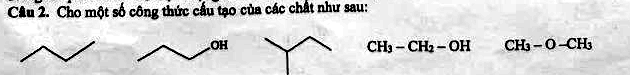
\includegraphics[width=0.85\textwidth]{images_danghuytru_ma102/structures_p2_c2_clean.png}
\end{center}
\choiceTF
{\True Công thức cấu tạo (2) và (4) biểu diễn cùng một chất.}
{\True Chất (2) và (4) có tính chất hoá học tương tự nhau.}
{\True Chất (4) và (5) là đồng phân của nhau.}
{\True Chất (1) và (3) là hydrocarbon mạch hở không phân nhánh..}
\loigiai{
$\bullet$ Ý a: \textbf{SAI}. Chất (2) là propan-1-ol ($\ce{C3H7OH}$), chất (4) là ethanol ($\ce{C2H5OH}$), là 2 chất khác nhau.\\
$\bullet$ Ý b: \textbf{ĐÚNG}. Cả 2 đều là alcohol no, đơn chức, mạch hở thuộc cùng một dãy đồng đẳng nên có tính chất tương tự nhau.\\
$\bullet$ Ý c: \textbf{ĐÚNG}. Cả 2 đều có cùng CTPT $\ce{C2H6O}$ nhưng khác CTCT nên là đồng phân của nhau.\\
$\bullet$ Ý d: \textbf{SAI}. Chất (3) là isobutane có mạch carbon phân nhánh (nhánh methyl tại C2).
}
\end{ex}

\vspace{6pt}
{\bfseries\color{mainGreen} Phần III: Trắc nghiệm trả lời ngắn (1,0 điểm).}
\textit{Học sinh trả lời từ câu 1 đến câu 4.}
\vspace{4pt}
\begin{ex}
Cho 6 hợp chất hữu cơ có công thức phân tử lần lượt là: $\ce{C2H6O}$, $\ce{C2H4O2}$, $\ce{C3H6O3}$, $\ce{C3H6O2}$, $\ce{C4H8O2}$, $\ce{C6H12O6}$. Có bao nhiêu hợp chất hữu cơ \textbf{không có} công thức đơn giản nhất là $\ce{CH2O}$?
\par\textbf{Trả lời:} \textbf{\color{hfRed}3}
\loigiai{
- $\ce{C2H6O}$: CTĐGN là $\ce{C2H6O}$ (khác $\ce{CH2O}$) $\rightarrow$ Thỏa mãn (1).\\
- $\ce{C2H4O2}$: CTĐGN là $\ce{CH2O}$.\\
- $\ce{C3H6O3}$: CTĐGN là $\ce{CH2O}$.\\
- $\ce{C3H6O2}$: CTĐGN là $\ce{C3H6O2}$ (khác $\ce{CH2O}$) $\rightarrow$ Thỏa mãn (2).\\
- $\ce{C4H8O2}$: CTĐGN là $\ce{C2H4O}$ (khác $\ce{CH2O}$) $\rightarrow$ Thỏa mãn (3).\\
- $\ce{C6H12O6}$: CTĐGN là $\ce{CH2O}$.\\
Vậy có 3 hợp chất không có CTĐGN là $\ce{CH2O}$.
}
\end{ex}
\begin{ex}
Trộn 200 mL dung dịch gồm $\ce{HCl}$ 0,1M và $\ce{H2SO4}$ 0,05M vào 300 mL dung dịch $\ce{Ba(OH)2}$ có nồng độ $a\text{ mol/L}$ thu được có $\text{pH} = 13$. Giá trị của $a$ là \textit{(Kết quả làm tròn đến hàng phần trăm)}.
\par\textbf{Trả lời:} \textbf{\color{hfRed}0,15}
\loigiai{
- $V = 200 + 300 = 500\text{ mL} = 0{,}5\text{ L}$.\\
- $\text{pH} = 13 \Rightarrow [\ce{OH-}]_{\text{dư}} = 10^{-1} = 0{,}1\text{ M} \Rightarrow n_{\ce{OH-}(\text{dư})} = 0{,}1 \times 0{,}5 = 0{,}05\text{ mol}$.\\
- $n_{\ce{H+}} = 0{,}2 \times 0{,}1 + 0{,}2 \times 0{,}05 \times 2 = 0{,}04\text{ mol}$.\\
- $n_{\ce{OH-}(\text{ban đầu})} = 0{,}3 \times 2a = 0{,}6a\text{ mol}$.\\
- Ta có: $n_{\ce{OH-}(\text{dư})} = n_{\ce{OH-}(\text{bđ})} - n_{\ce{H+}} \Leftrightarrow 0{,}05 = 0{,}6a - 0{,}04 \Leftrightarrow 0{,}6a = 0{,}09 \Leftrightarrow a = 0{,}15\text{ M}$.
}
\end{ex}
\begin{ex}
Các cách làm sau đây, cách nào sử dụng phương pháp chiết?
\begin{enumerate}[label=(\arabic*),leftmargin=20pt,itemsep=0pt]
\item Giã lá cây chàm, cho vào nước, lọc lấy dung dịch màu để nhuộm sợi, vải.
\item Dùng nước sôi để pha trà, cà phê.
\item Ngâm rượu thuốc.
\item Làm đường cát, đường phèn từ nước mía.
\end{enumerate}
\par\textbf{Trả lời:} \textbf{\color{hfRed}3}
\loigiai{
Các cách (1), (2), (3) đều dùng dung môi thích hợp để hòa tan chất cần tách ra khỏi chất rắn, đó là phương pháp chiết lỏng - rắn. Cách (4) là phương pháp kết tinh. Vậy có 3 cách sử dụng phương pháp chiết (gồm 1, 2, 3).
}
\end{ex}
\begin{ex}
Có một loại quặng pyrite chứa 84\% $\ce{FeS2}$. Nếu mỗi ngày nhà máy sản xuất 10 tấn sulfuric acid 98\% thì cần $m$ tấn quặng pyrite trên và biết hiệu suất của cả quá trình sản xuất $\ce{H2SO4}$ là 60\%. Giá trị của $m$ là \textit{(Kết quả làm tròn đến hàng phần mười)}.
\par\textbf{Trả lời:} \textbf{\color{hfRed}11,9}
\loigiai{
- $m_{\ce{H2SO4}} = 10 \times 98\% = 9{,}8\text{ tấn} \Rightarrow n_{\ce{H2SO4}} = \frac{9{,}8}{98} = 0{,}1\text{ Mmol}$.\\
- Sơ đồ bảo toàn S: $\ce{FeS2 -> 2H2SO4} \Rightarrow n_{\ce{FeS2(lt)}} = 0{,}05\text{ Mmol}$.\\
- Hiệu suất $H = 60\% \Rightarrow n_{\ce{FeS2(tt)}} = \frac{0{,}05}{0{,}6} = \frac{1}{12}\text{ Mmol}$.\\
- $m_{\ce{FeS2(tt)}} = \frac{1}{12} \times 120 = 10\text{ tấn}$.\\
- $m_{\text{quặng}} = \frac{10}{84\%} \approx 11{,}9048\text{ tấn} \approx 11{,}9\text{ tấn}$.
}
\end{ex}

\vspace{6pt}
{\large\bfseries\color{mainGreen} B. TỰ LUẬN (3,0 điểm)}

\vspace{3pt}
\textbf{Câu 1 (1,0 điểm):} Hoàn thành phương trình hóa học của các phản ứng sau?
\begin{enumerate}[label=\alph*),leftmargin=25pt,itemsep=2pt]
\item $\ce{KOH + H2SO4 ->}$
\item $\ce{H2SO4\text{ loãng} + Fe2O3 ->}$
\item $\ce{NO2 + O2 + H2O ->}$
\item $\ce{NH4Cl + NaOH ->}$
\end{enumerate}

\begin{tcolorbox}[colback=white,colframe=solBlue,arc=2mm,boxrule=0.5pt,title=\textbf{Lời giải Câu 1 (Tự luận)}]
a) $\ce{2KOH + H2SO4 -> K2SO4 + 2H2O}$\\
b) $\ce{3H2SO4(lo\~ang) + Fe2O3 -> Fe2(SO4)3 + 3H2O}$\\
c) $\ce{4NO2 + O2 + 2H2O -> 4HNO3}$\\
d) $\ce{NH4Cl + NaOH -> NaCl + NH3 ^ + H2O}$
\end{tcolorbox}

\vspace{4pt}
\textbf{Câu 2 (1,0 điểm):} Camphor (có trong cây long não) là một chất rắn kết tinh màu trắng hay trong suốt giống như sáp với mùi thơm đặc trưng, thường dùng trong y học. Phần trăm khối lượng các nguyên tố trong camphor lần lượt là 78,94\% carbon, 10,53\% hydrogen và 10,53\% oxygen.

\begin{minipage}[t]{0.52\textwidth}
1) Lập công thức đơn giản nhất của camphor.\\
b) Xác định công thức phân tử của camphor biết phổ MS của camphor được cho như hình bên.
\end{minipage}
\hfill
\begin{minipage}[t]{0.45\textwidth}
\centering
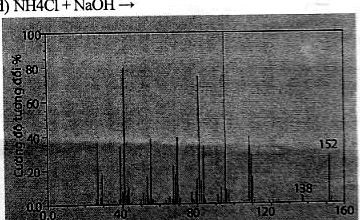
\includegraphics[width=0.95\textwidth]{images_danghuytru_ma102/ms_camphor_clean.png}
\end{minipage}

\begin{tcolorbox}[colback=white,colframe=solBlue,arc=2mm,boxrule=0.5pt,title=\textbf{Lời giải Câu 2 (Tự luận)}]
\textbf{1) Lập công thức đơn giản nhất của camphor:}\\
Đặt công thức đơn giản nhất là $\ce{C}_x\ce{H}_y\ce{O}_z$.\\
Tỉ lệ số mol:
\[
x : y : z = \frac{78{,}94}{12} : \frac{10{,}53}{1} : \frac{10{,}53}{16} = 6{,}578 : 10{,}53 : 0{,}658 \approx 10 : 16 : 1
\]
Vậy công thức đơn giản nhất của camphor là $\ce{C10H16O}$.\\[4pt]
\textbf{b) Xác định công thức phân tử của camphor:}\\
Công thức phân tử có dạng $(\ce{C10H16O})_n \Rightarrow M = 152n$.\\
Trên phổ MS, peak ion phân tử $[M^+]$ có $m/z = 152 \Rightarrow M = 152\text{ g/mol} \Rightarrow n = 1$.\\
Vậy công thức phân tử của camphor là $\ce{C10H16O}$.
\end{tcolorbox}

\vspace{4pt}
\textbf{Câu 3 (1,0 điểm):} Hàm lượng cho phép của sulfur trong nhiên liệu là 0,3\% về khối lượng. Để xác định hàm lượng sulfur trong một loại nhiên liệu người ta lấy 100,0 gam nhiên liệu đó và đốt cháy hoàn toàn. Khí tạo thành chỉ chứa carbon dioxide, sulfur dioxide và hơi nước được dẫn vào nước tạo ra 500,0 ml dung dịch. Biết rằng tất cả sulfur dioxide đã tan vào dung dịch. Lấy 10,0 ml dung dịch này cho tác dụng với dung dịch $\ce{KMnO4}\ 5{,}00\cdot 10^{-3}\text{ mol/L}$ thì thể tích dung dịch $\ce{KMnO4}$ cần dùng là 12,5 mL. Tính phần trăm khối lượng của sulfur trong nhiên liệu trên?\\
\textit{(Cho NTK các nguyên tố: C: 12, H: 1, O: 16, Ba: 137, S: 32)}

\begin{tcolorbox}[colback=white,colframe=solBlue,arc=2mm,boxrule=0.5pt,title=\textbf{Lời giải Câu 3 (Tự luận)}]
- Phương trình phản ứng chuẩn độ:
\[
\ce{5SO2 + 2KMnO4 + 2H2O -> K2SO4 + 2MnSO4 + 2H2SO4}
\]
- Số mol $\ce{KMnO4}$ phản ứng trong 10,0 mL dung dịch:
\[
n_{\ce{KMnO4}} = 0{,}0125 \times 5{,}00\cdot 10^{-3} = 6{,}25\cdot 10^{-5}\text{ mol}
\]
- Theo phương trình:
\[
n_{\ce{SO2(10 mL)}} = \frac{5}{2} \times 6{,}25\cdot 10^{-5} = 1{,}5625\cdot 10^{-4}\text{ mol}
\]
- Tổng số mol $\ce{SO2}$ trong 500,0 mL dung dịch:
\[
n_{\ce{SO2(tổng)}} = 1{,}5625\cdot 10^{-4} \times \frac{500{,}0}{10{,}0} = 7{,}8125\cdot 10^{-3}\text{ mol}
\]
- Bảo toàn nguyên tố S:
\[
n_{\ce{S}} = n_{\ce{SO2}} = 7{,}8125\cdot 10^{-3}\text{ mol} \Rightarrow m_{\ce{S}} = 7{,}8125\cdot 10^{-3} \times 32 = 0{,}25\text{ g}
\]
- Phần trăm khối lượng sulfur trong nhiên liệu:
\[
\%m_{\ce{S}} = \frac{0{,}25}{100{,}0} \times 100\% = 0{,}25\%
\]
- Nhận xét: $0{,}25\% \le 0{,}3\%$, đạt tiêu chuẩn an toàn cho phép.
\end{tcolorbox}

\vspace{6pt}
\begin{center}
\textbf{\large ---------- HẾT ----------}
\end{center}

\end{document}
